\newpage
\section{Durchführung}
Es wurden ein Oszilloskop und eine Spannungsquelle sowie verschiedene Kondensatoren, Spulen, und Widerstände zur Verfügung gestellt.
Da Aufgabenteile b) c) und d) aufgrund technischer Fehler nicht selbst durchgeführt werden konnten, wurden die Daten aus (\ref{tab:ab8}), (\ref{tab:ab9}), (\ref{tab:ac10}), (\ref{tab:ac18}), (\ref{tab:ad10}) und (\ref{tab:ad18}) zur Verfügung gestellt.

\subsection{Aufgabe a)}
Um die unbekannten Widerstände zu messen, wird die Wheatstone'sche Brückenschaltung nach Abbildung (\ref{fig:wheat}) aufgebaut.
Die Frequenz bleibt dabei die ganze Zeit bei 1500 Hz

\begin{enumerate}
\item \textbf{Wert 13}

Zur Bestimmung vom unbekannten Widerstand Wert 13 wird $\text{R}_2 = 664 \Omega$ gewählt.
Nun wird am Potentiometer so lange gedreht, bis die Spannung minimal wird.
Dies war bei $\text{R}_3 = 317,5 \Omega$ und $\text{R}_4 = 682,5 \Omega$ der Fall.

\noindent
Das Vorgehen wird mit einem anderen Widerstand $\text{R}_2 =1\text{k} \Omega$ wiederholt.

Dann ergibt sich $\text{R}_3 = 241 \Omega$ und $\text{R}_4 = 759 \Omega$.

\item \textbf{Wert 14}

Dies wurde analog für einen zweiten unbekannten Widerstand Wert 14 durchgeführt.

Für $\text{R}_2 = 664 \Omega$ ergibt sich $\text{R}_3 = 573,5 \Omega$ und für $\text{R}_4 = 426,5 \Omega$.

Für $\text{R}_2 = 1\text{k} \Omega$ ergibt sich $\text{R}_3 = 471 \Omega$ und für $\text{R}_4 = 529 \Omega$.
\end{enumerate}


\subsection{Aufgabe b)}

Durch eine Kapazitätsmessbrücke nach (\ref{fig:kap}) werden die zwei unbekannten Kapazitäten Wert 8 und Wert 9 gemessen.

\begin{enumerate}
\item \textbf{Wert 8}

\begin{table}
\centering
\begin{tabular}{c c c c c}
\toprule
{Messung} & {$\text{C}_2 \mathbin{/} \si{\nano\farad}$} &{$ \text{R}_2 \mathbin{/} \si{\ohm} $} & {$ \text{R}_3 \mathbin{/} \si{\ohm} $} & {$ \text{R}_4 \mathbin{/} \si{\ohm} $} \\
\midrule
1 & 450 & 371 & 606 & 394 \\
2 & 399 & 418 & 578 & 422 \\
3 & 597 & 278 & 673 & 327 \\
\bottomrule
\end{tabular}
\caption{Daten für Wert 8.}
\label{tab:ab8}
\end{table}

\newpage

\item \textbf{Wert 9}

\begin{table}
\centering
\begin{tabular}{c c c c c}
\toprule
{Messung} & {$\text{C}_2 \mathbin{/} \si{\nano\farad}$} &{$ \text{R}_2 \mathbin{/} \si{\ohm} $} & {$ \text{R}_3 \mathbin{/} \si{\ohm} $} & {$ \text{R}_4 \mathbin{/} \si{\ohm} $} \\
\midrule
1 & 450 & 466 & 511 & 489 \\
2 & 399 & 524 & 481 & 519 \\
3 & 597 & 352 & 581 & 419 \\
\bottomrule
\end{tabular}
\caption{Daten für Wert 9.}
\label{tab:ab9}
\end{table}

\end{enumerate}

\subsection{Aufgabe c)}

Hier sollen mit einer Induktivitätsbrücke nach (\ref{fig:induktiv}) die zwei unbekannten Induktivitäten Wert 10 und Wert 18 gemessen werden.

\begin{enumerate}
\item \textbf{Wert 10}

\begin{table}
\centering
\begin{tabular}{c c c c c}
\toprule
{Messung} & {$\text{L}_2 \mathbin{/} \si{\milli\henry}$} &{$ \text{R}_2 \mathbin{/} \si{\ohm} $} & {$ \text{R}_3 \mathbin{/} \si{\ohm} $} & {$ \text{R}_4 \mathbin{/} \si{\ohm} $} \\
\midrule
1 & 14,6 & 45 & 907 & 83 \\
2 & 20,1 & 57 & 875 & 125 \\
3 & 27,5 & 85 & 837 & 163 \\
\bottomrule
\end{tabular}
\caption{Daten für Wert 10.}
\label{tab:ac10}
\end{table}



\item \textbf{Wert 18}

\begin{table}
\centering
\begin{tabular}{c c c c c}
\toprule
{Messung} & {$\text{L}_2 \mathbin{/} \si{\milli\henry}$} &{$ \text{R}_2 \mathbin{/} \si{\ohm} $} & {$ \text{R}_3 \mathbin{/} \si{\ohm} $} & {$ \text{R}_4 \mathbin{/} \si{\ohm} $} \\
\midrule
1 & 14,6 & 108 & 775 & 225 \\
2 & 20,1 & 143 & 715 & 285 \\
3 & 27,5 & 197 & 648 & 352 \\
\bottomrule
\end{tabular}
\caption{Daten für Wert 18.}
\label{tab:ac18}
\end{table}

\end{enumerate}

\newpage
\subsection{Aufgabe d)}

Nun soll die Vermessung der unbekannten Induktivitäten nochmal auf eine andere Art gemessen werden.
Diesmal duch die Maxwell Brücke nach (\ref{fig:max}). 

\begin{enumerate}
\item \textbf{Wert 10}

\begin{table}
\centering
\begin{tabular}{c c c c }
\toprule
{Messung} &{$ \text{R}_2 \mathbin{/} \si{\ohm} $} & {$ \text{R}_3 \mathbin{/} \si{\ohm} $} & {$ \text{R}_4 \mathbin{/} \si{\ohm} $} \\
\midrule
1 & 100 & 347 & 829 \\
2 & 664 & 523 & 829 \\
3 & 332 & 1036 & 829 \\
\bottomrule
\end{tabular}
\caption{Daten für Wert 10.}
\label{tab:ad10}
\end{table}



\item \textbf{Wert 18}

\begin{table}
\centering
\begin{tabular}{c c c c }
\toprule
{Messung} & {$ \text{R}_2 \mathbin{/} \si{\ohm} $} & {$ \text{R}_3 \mathbin{/} \si{\ohm} $} & {$ \text{R}_4 \mathbin{/} \si{\ohm} $} \\
\midrule
1 & 100 & 128 & 347 \\
2 & 664 & 193 & 349 \\
3 & 332 & 382 & 348 \\
\bottomrule
\end{tabular}
\caption{Daten für Wert 18.}
\label{tab:ad18}
\end{table}

\end{enumerate}

\newpage
\subsection{Aufgabe e)}

\begin{figure}
            \centering
               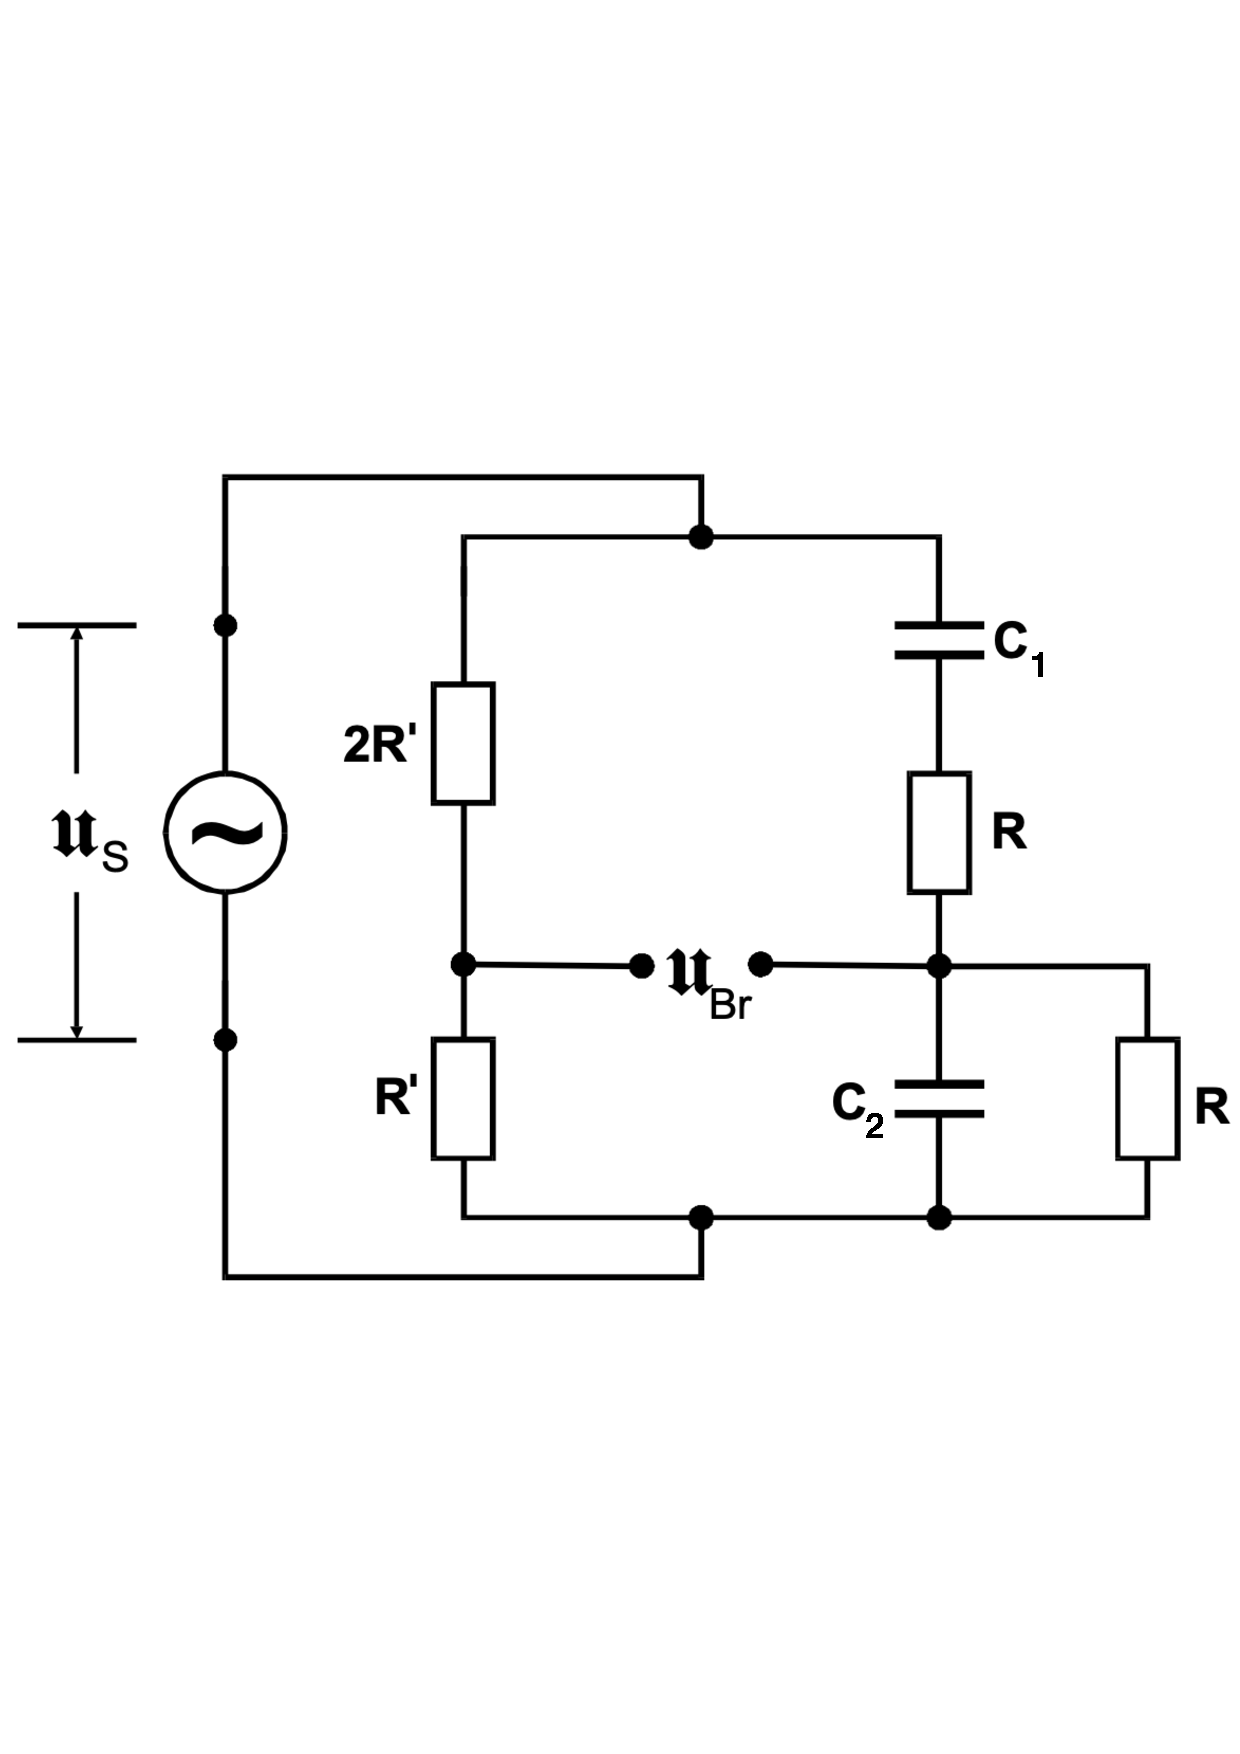
\includegraphics[height=7cm]{wiene.pdf}
               \caption{Schaltung einer Wien-Robinson-Brücke mit 2 verschiedenen Kapazitäten.}
               \label{fig:wiene}
        \end{figure}


\noindent
Danach sollte die Frequenzabhängigkeit der Brückenspannung einer Wien-Robinson-Brücke untersucht und mit der Theorie verglichen werden.
Hierzu wird die Brücke nach (\ref{fig:wiene}) aufgebaut, mit

\begin{align*}
\text{R}' &= 500\Omega\\
\text{R} &= 1\text{k}\Omega\\
\text{C}_1 &= 399 \si{\nano\farad}\\
\text{C}_2 &= 450 \si{\nano\farad}.
\end{align*}

\noindent
Da keine zwei gleichen Kapazitäten zur Verfügung standen, wurden möglichst gleichgroße verwendet.
Nun wird die Frequenz variiert und die dazugehörigen doppelten Amplituden gemessen.
Diese konnten auf dem Oszilloskop beobachtet und mit dem Cursor vermessen werden.
Folgende Werte wurden dabei ermittelt:


\begin{table}
\centering
\begin{tabular}{c c c}
\toprule
{$\text{f} \mathbin{/} \si{\hertz}$} &{$ 2\text{U}_\text{Br} \mathbin{/} \si{\volt} $} & {$ 2 \text{U}_\text{S} \mathbin{/} \si{\volt} $} \\
\midrule
20    & 6.44  & 20\\
36    & 6.32  & 20\\
45    & 6.20  & 20\\
60   &  6.00  & 20\\
75   &  5.68  & 20\\
90   &  5.40  & 20\\
105  &  5.00  & 20\\
120  &  4.68  & 20\\
135  &  4.24  & 20\\
150  &  3.92  & 20\\
200  &  2.80  & 20\\
300  &  1.07  & 20\\
340  &  0.520 & 20\\
375  &  0.282 & 20\\
370  &  0.308 & 20\\
380  &  0.308 & 20\\
400  &  0.412 & 20\\
420  &  0.580 & 20\\
440  &  0.784 & 20\\
480  &  1.14  & 20\\
500  &  1.32  & 20\\
650  &  2.38  & 20\\
750  &  2.94  & 20\\
900  &  3.60  & 20\\
1400 &  4.58  & 20\\
1700 &  5.32  & 20\\
8000 &  6.40  & 20\\
14000&  6.12  & 20\\
20000&  5.92  & 20\\
24000&  5.72  & 20\\
28000&  5.56  & 20\\
30000&  5.40  & 20\\
\bottomrule
\end{tabular}
\caption{Daten für doppelte Amplituden von $\text{U}_\text{Br}$ und $\text{U}_\text{S}$ bei variierten Frequenzen.}
\label{tab:ae}
\end{table}